\documentclass[aspectratio=169]{beamer}
\setbeamertemplate{navigation symbols}{}
\usepackage{color,amsmath,comment, subfigure}
\usepackage{booktabs}
\def\vf{\vfill}
\usepackage{url}

%\setbeameroption{show notes}

%%%%%%%%%%%%%%%%%%%%%%%%%%
\title[]{Class 11: Cascades and fads in cultural markets}
\author[]{Matthew J. Salganik}
\institute[]{Sociology 204: Social Networks\\Princeton University}
\date[]{
1/2: The puzzling nature of success in cultural markets
\vfill

\begin{flushleft}
\vspace{0.6in}

\includegraphics[width=0.1\textwidth]{figures/cc.png}
\end{flushleft}

}

\note{
Next year possibly have them predict experiment 3 which they have not seen
}

\begin{document}
%%%%%%%%%%%%%%%%%%%%%%%%%%%
\frame{\titlepage}
%%%%%%%%%%%%%%%%%%%%%%%%%%%
\begin{frame}

Review:
\begin{itemize}
\item sometimes small shocks get big and sometimes they don't
\pause
\item sequential behavior can lead to unexpected outcomes
\end{itemize}

\end{frame}
%%%%%%%%%%%%%%%%%%%%%%%
\begin{frame}

  \begin{columns}
    \column{0.4\textwidth}
     \begin{block}{}
       
\includegraphics[width=\textwidth]{figures/hp-cover.pdf}
     \end{block}

   \pause
   
   \column{0.6\textwidth}
     \begin{block}{}
       \begin{itemize}
         \item Wild success
         \item Rejected by eight publishers\\
       \end{itemize}
       This seems like a strange combination.
     \end{block}
  \end{columns}

\end{frame}
%%%%%%%%%%%%%%%%%%%%%%%%
\begin{frame}

  \begin{columns}
    \column{0.4\textwidth}
     \begin{block}{}
       
\includegraphics[width=\textwidth]{figures/star-wars}
     \end{block}
   
   \column{0.6\textwidth}
     \begin{block}{}
       \begin{itemize}
         \item Set box office records, won 6 Oscars, and launched a multi-billion dollar franchise
         \item Rejected by United Artists and Universal before being made by Fox
       \end{itemize}
     \end{block}
  \end{columns}

\end{frame}
%%%%%%%%%%%%
\begin{frame}

  \begin{columns}
    \column{0.4\textwidth}
     \begin{block}{}
       
\includegraphics[width=\textwidth]{figures/american-idol}
     \end{block}

   \column{0.6\textwidth}
     \begin{block}{}
       \begin{itemize}
         \item One of the most popular shows of the decade
         \item Rejected by ABC, CBS, and NBC before being picked up by Fox
       \end{itemize}
     \end{block}
  \end{columns}

\end{frame}

%%%%%%%%%%%%%%%%
\begin{frame}

  Puzzling nature of success for cultural objects (books, movies, piece of art, music)
  \vspace{0.2in}
  \begin{itemize}
    \item<1-> extreme inequality in the success of objects \\
    \item <2-> unpredictability in the success of objects \\
  \end{itemize}

\end{frame}
%%%%%%%%%%%%%%%%%%%%%%%%%%%%%%%
\begin{frame} 

\textbf{Psychological explanation:}\\
People agree on what's good, but people are hard to predict\\

\vspace{0.2in}

\textbf{Sociological explanation:}\\
The collective outcomes of inequality and unpredictability of success both arise from an individual-level process of social influence\\

\begin{figure}
  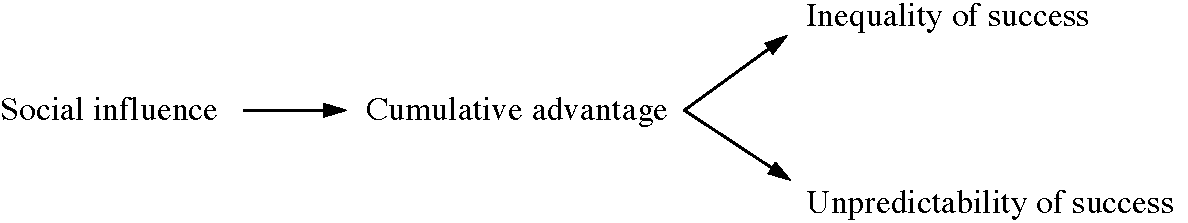
\includegraphics[width = 0.8\textwidth]{figures/musiclab_model}
\end{figure}

\end{frame}

%%%%%%%%%%%%%%%%%%%%%%%%%%%%%%%%%%%
\begin{frame}

\begin{figure}
  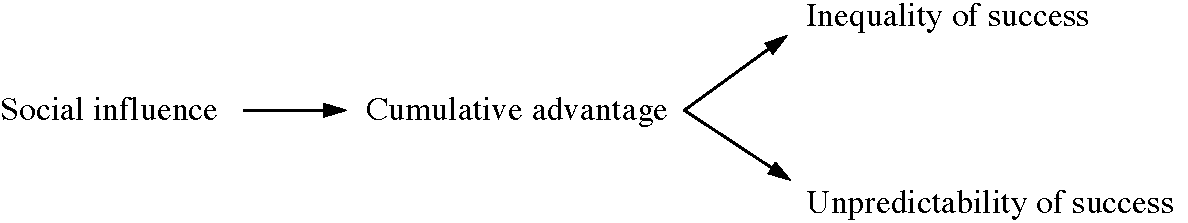
\includegraphics[width = 0.8\textwidth]{figures/musiclab_model}
\end{figure}

Problems with observational data:
\begin{itemize}
\item don't know what would have happened without social influence
\pause
\item can't see multiple ``histories'' to observe unpredictability
\end{itemize}

\end{frame}

%%%%%%%%%%%%%%%%%%%%%%%%%%%%%%%%%%%
\begin{frame}

Instead of using observational data we are going to run an experiment because
\begin{itemize}
\item can control the information that people have about the behavior of others
\pause
\item can run the same process multiple times under exactly the same conditions, allows us to see multiple ``histories''
\end{itemize}

\vspace{0.2in}
But, this experiment is different from most,
\begin{itemize}
\item experiments in psychology and economics have \textbf{individual}
as unit of analysis, require \textbf{hundreds} of participants 
\item these sociological experiments have \textbf{collective outcome}
as unit of analysis, require \textbf{thousands} of participants
\end{itemize}
Web-based experiment allow for such large sample sizes because each additional participant has no cost (total $n= 27,267$)\\

\end{frame}
%%%%%%%%%%%%%%%%%%%%%%%%%%%%%%%%%%%
\begin{frame}

\begin{center}
\includegraphics<1>[width = 0.85\textwidth]{figures/zero_variable_cost_1}
\includegraphics<2>[width = 0.85\textwidth]{figures/zero_variable_cost_2}
\end{center}

\end{frame}
%%%%%%%%%%%%%%%%%%%%%%%%%%%%
\begin{frame}

\begin{figure}
  \centering
  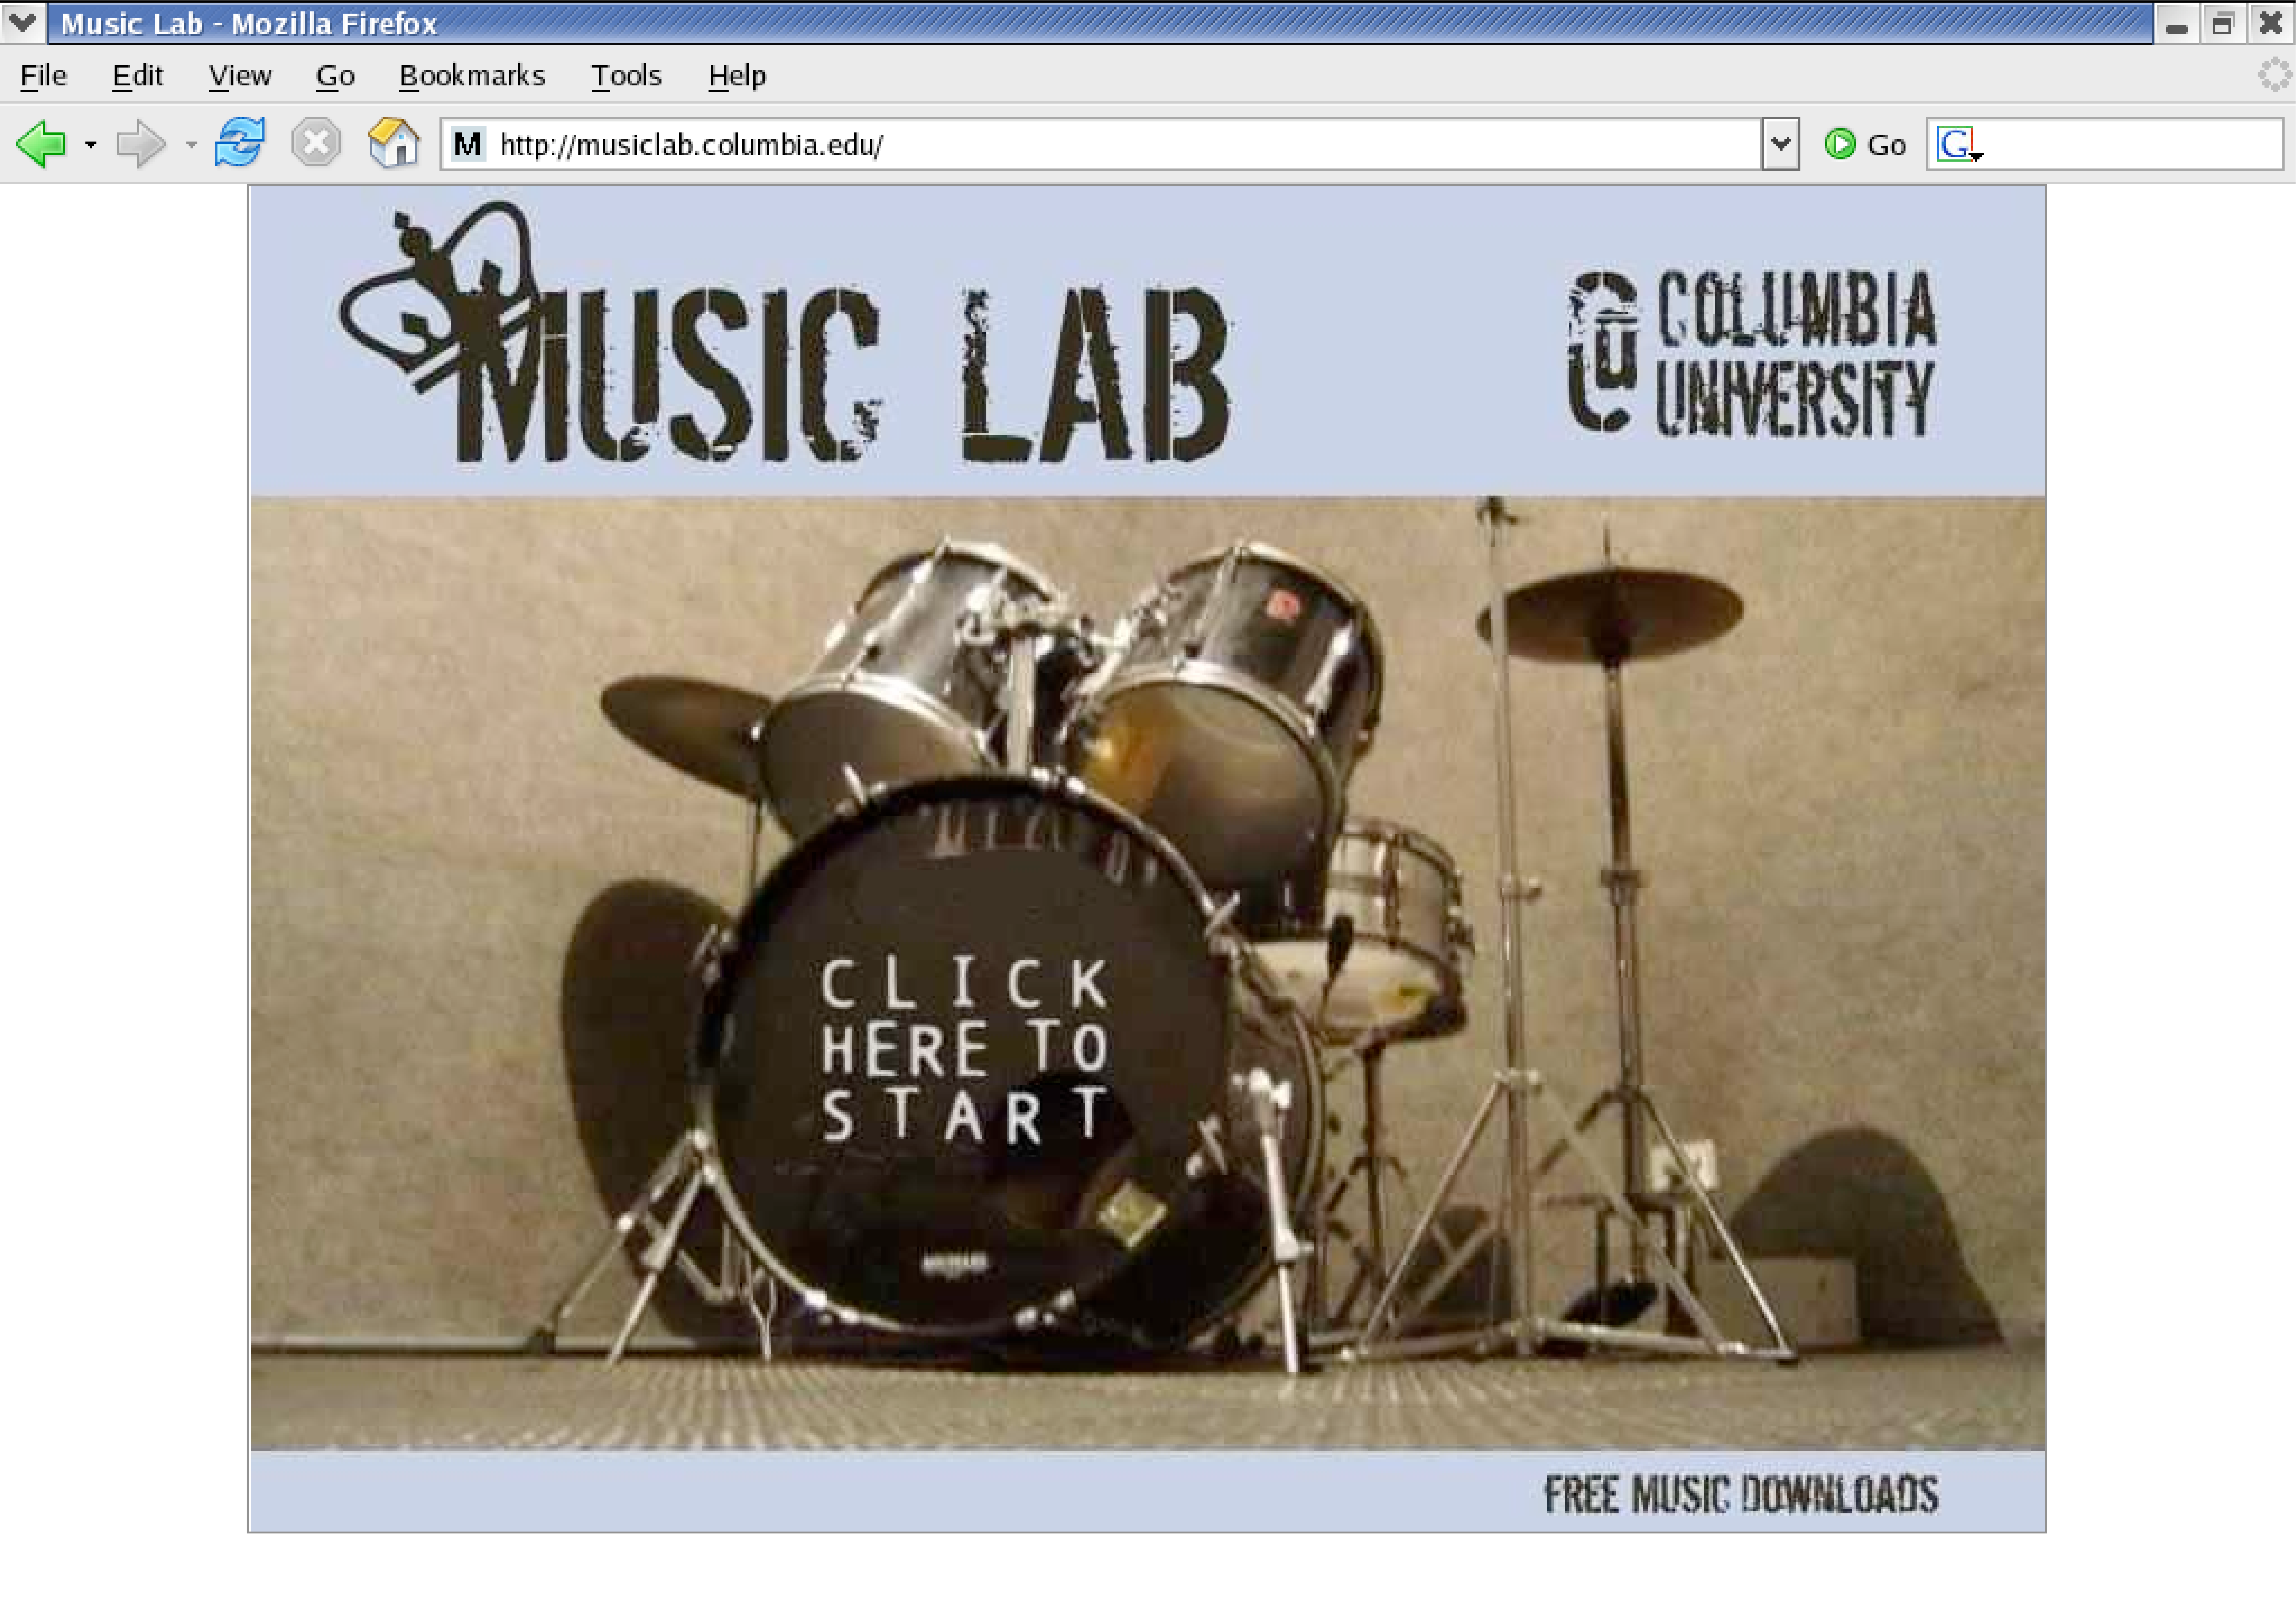
\includegraphics[width = 0.9\textwidth]{figures/splashscreen}
\end{figure}

\end{frame}
%%%%%%%%%%%%%%%%%%%%%%%%%%%%%%%%%
\begin{frame}

\begin{figure}
  \centering
  \includegraphics[width = 0.9\textwidth]{figures/info-v1-cut}
\end{figure}

\end{frame}
%%%%%%%%%%%%%%%%%%%%%%%%%%%%%%%%%
\begin{frame} 

\begin{figure}
  \centering
  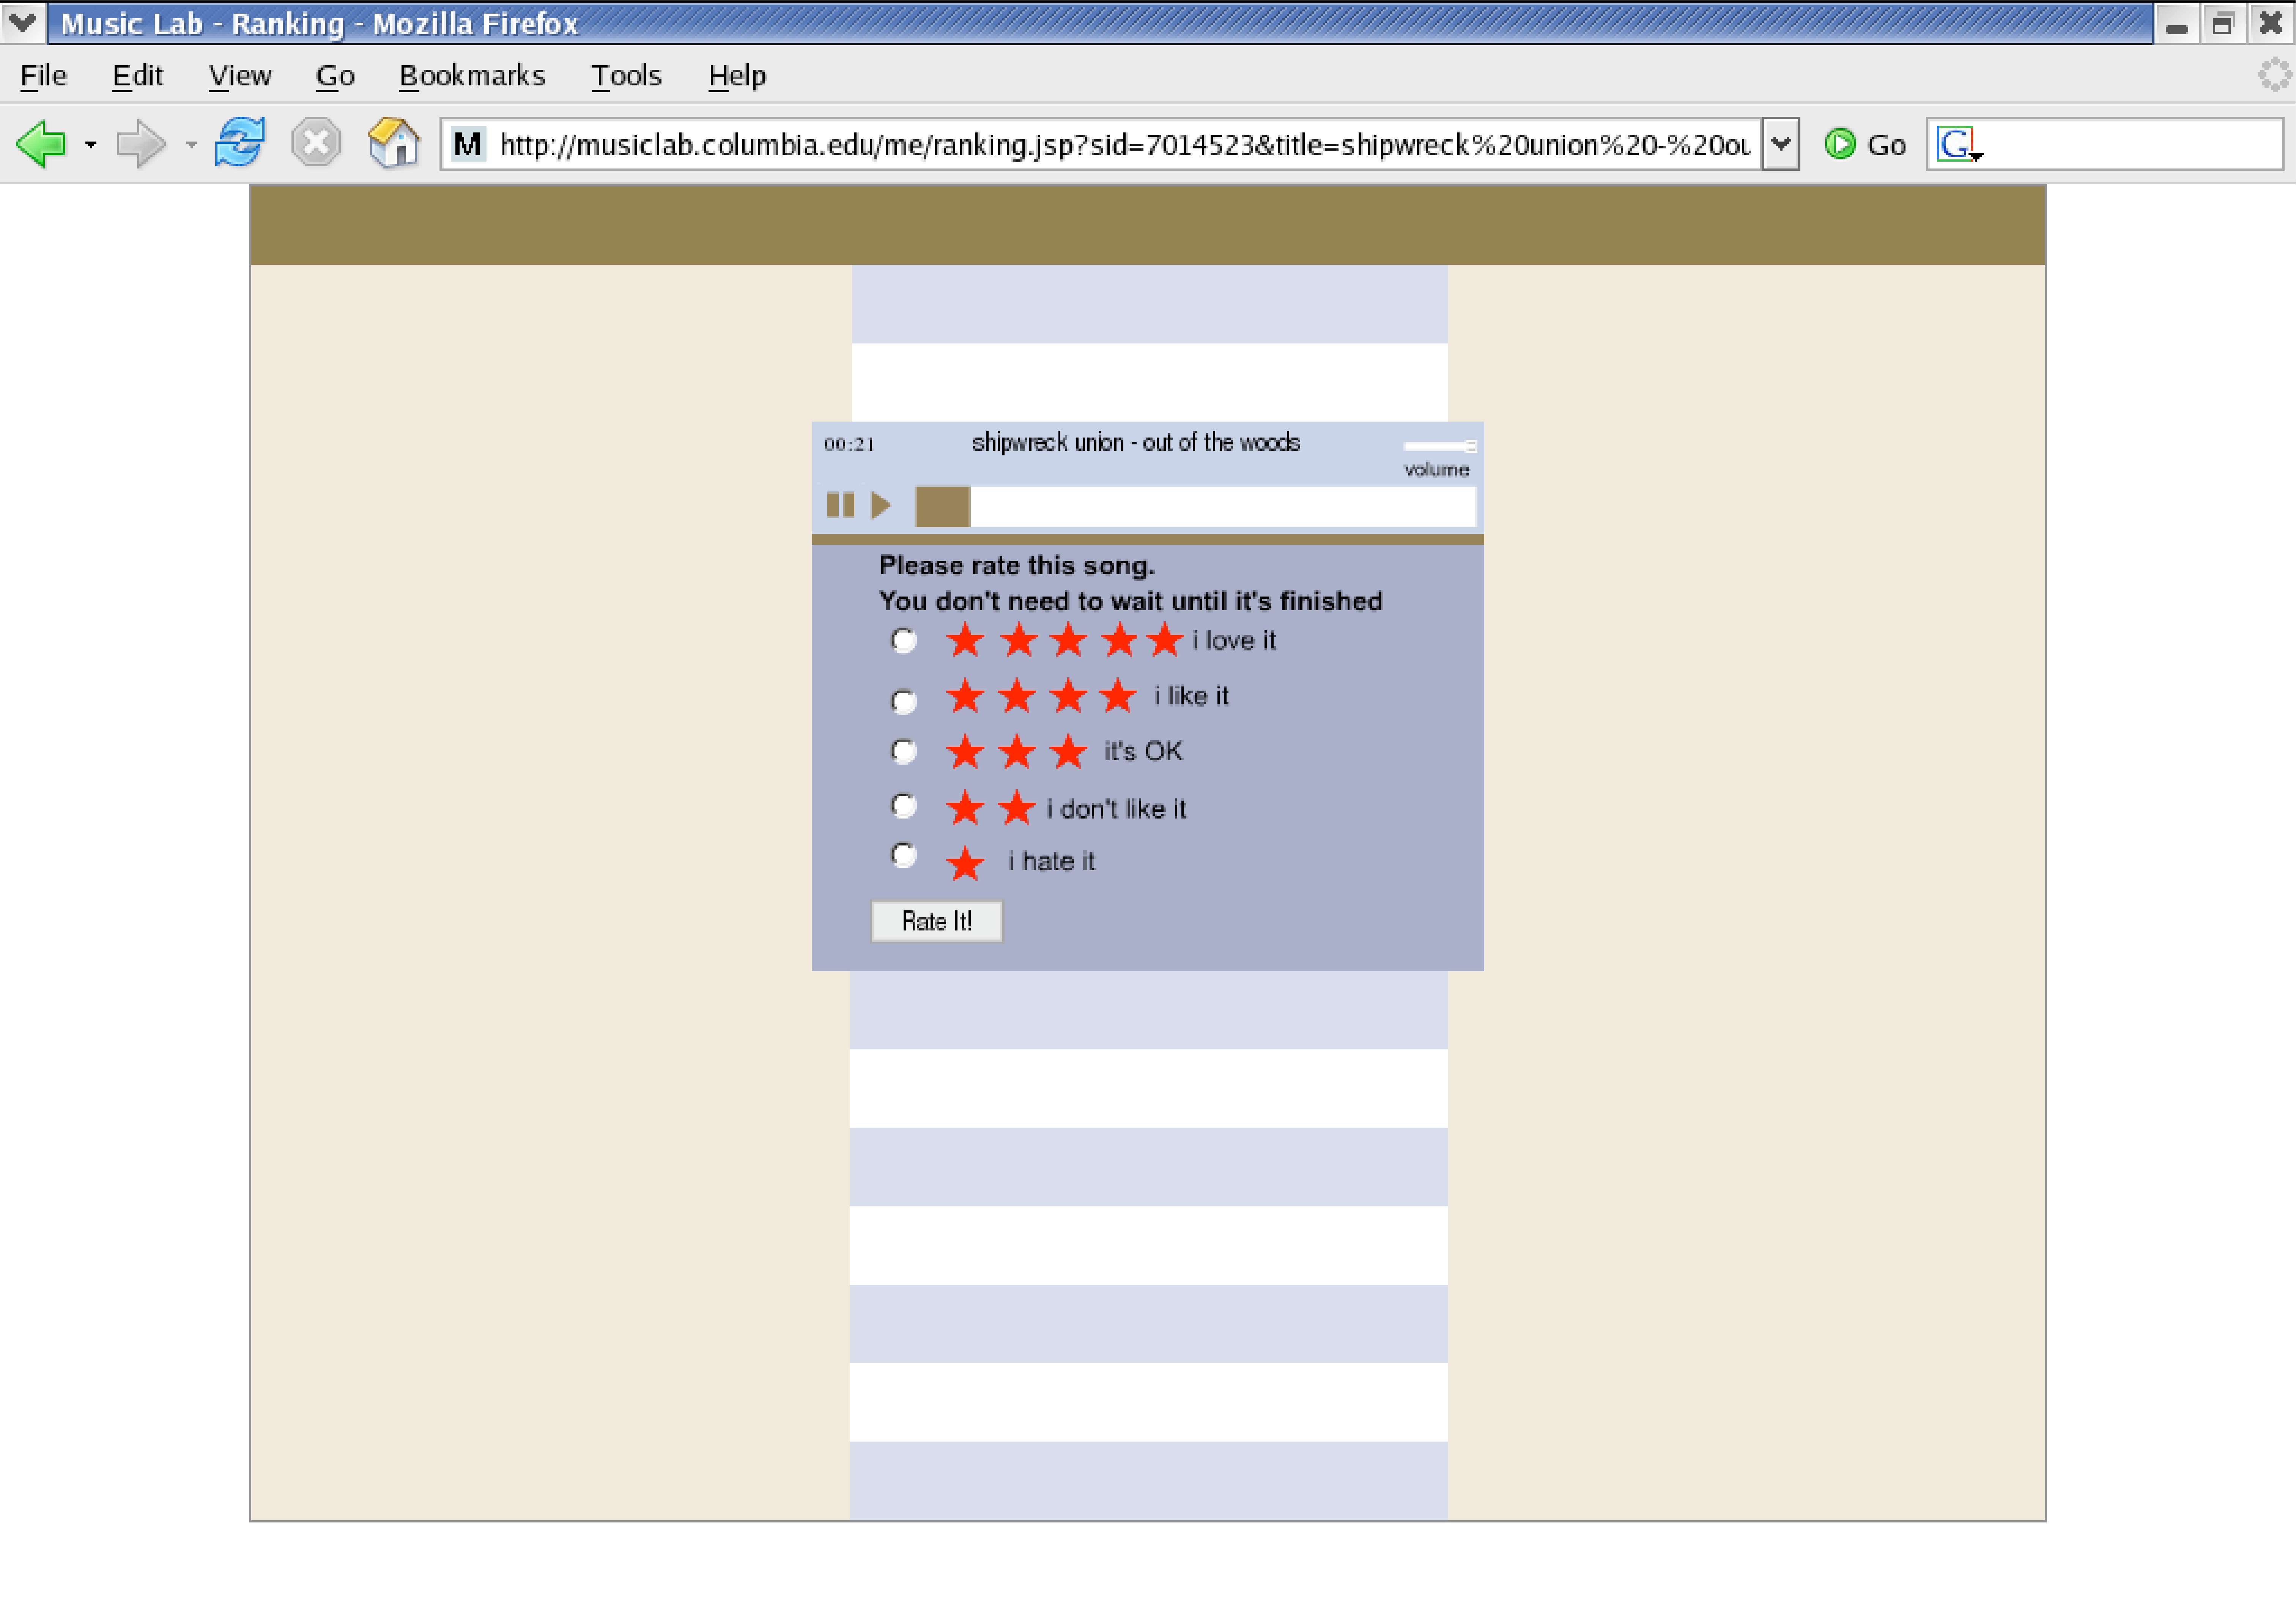
\includegraphics[width = 0.9\textwidth]{figures/listenscreen}
\end{figure}

\end{frame}
%%%%%%%%%%%%%%%%%%%%%%%%%%%%%%%%%
\begin{frame}

\begin{figure}
  \centering
  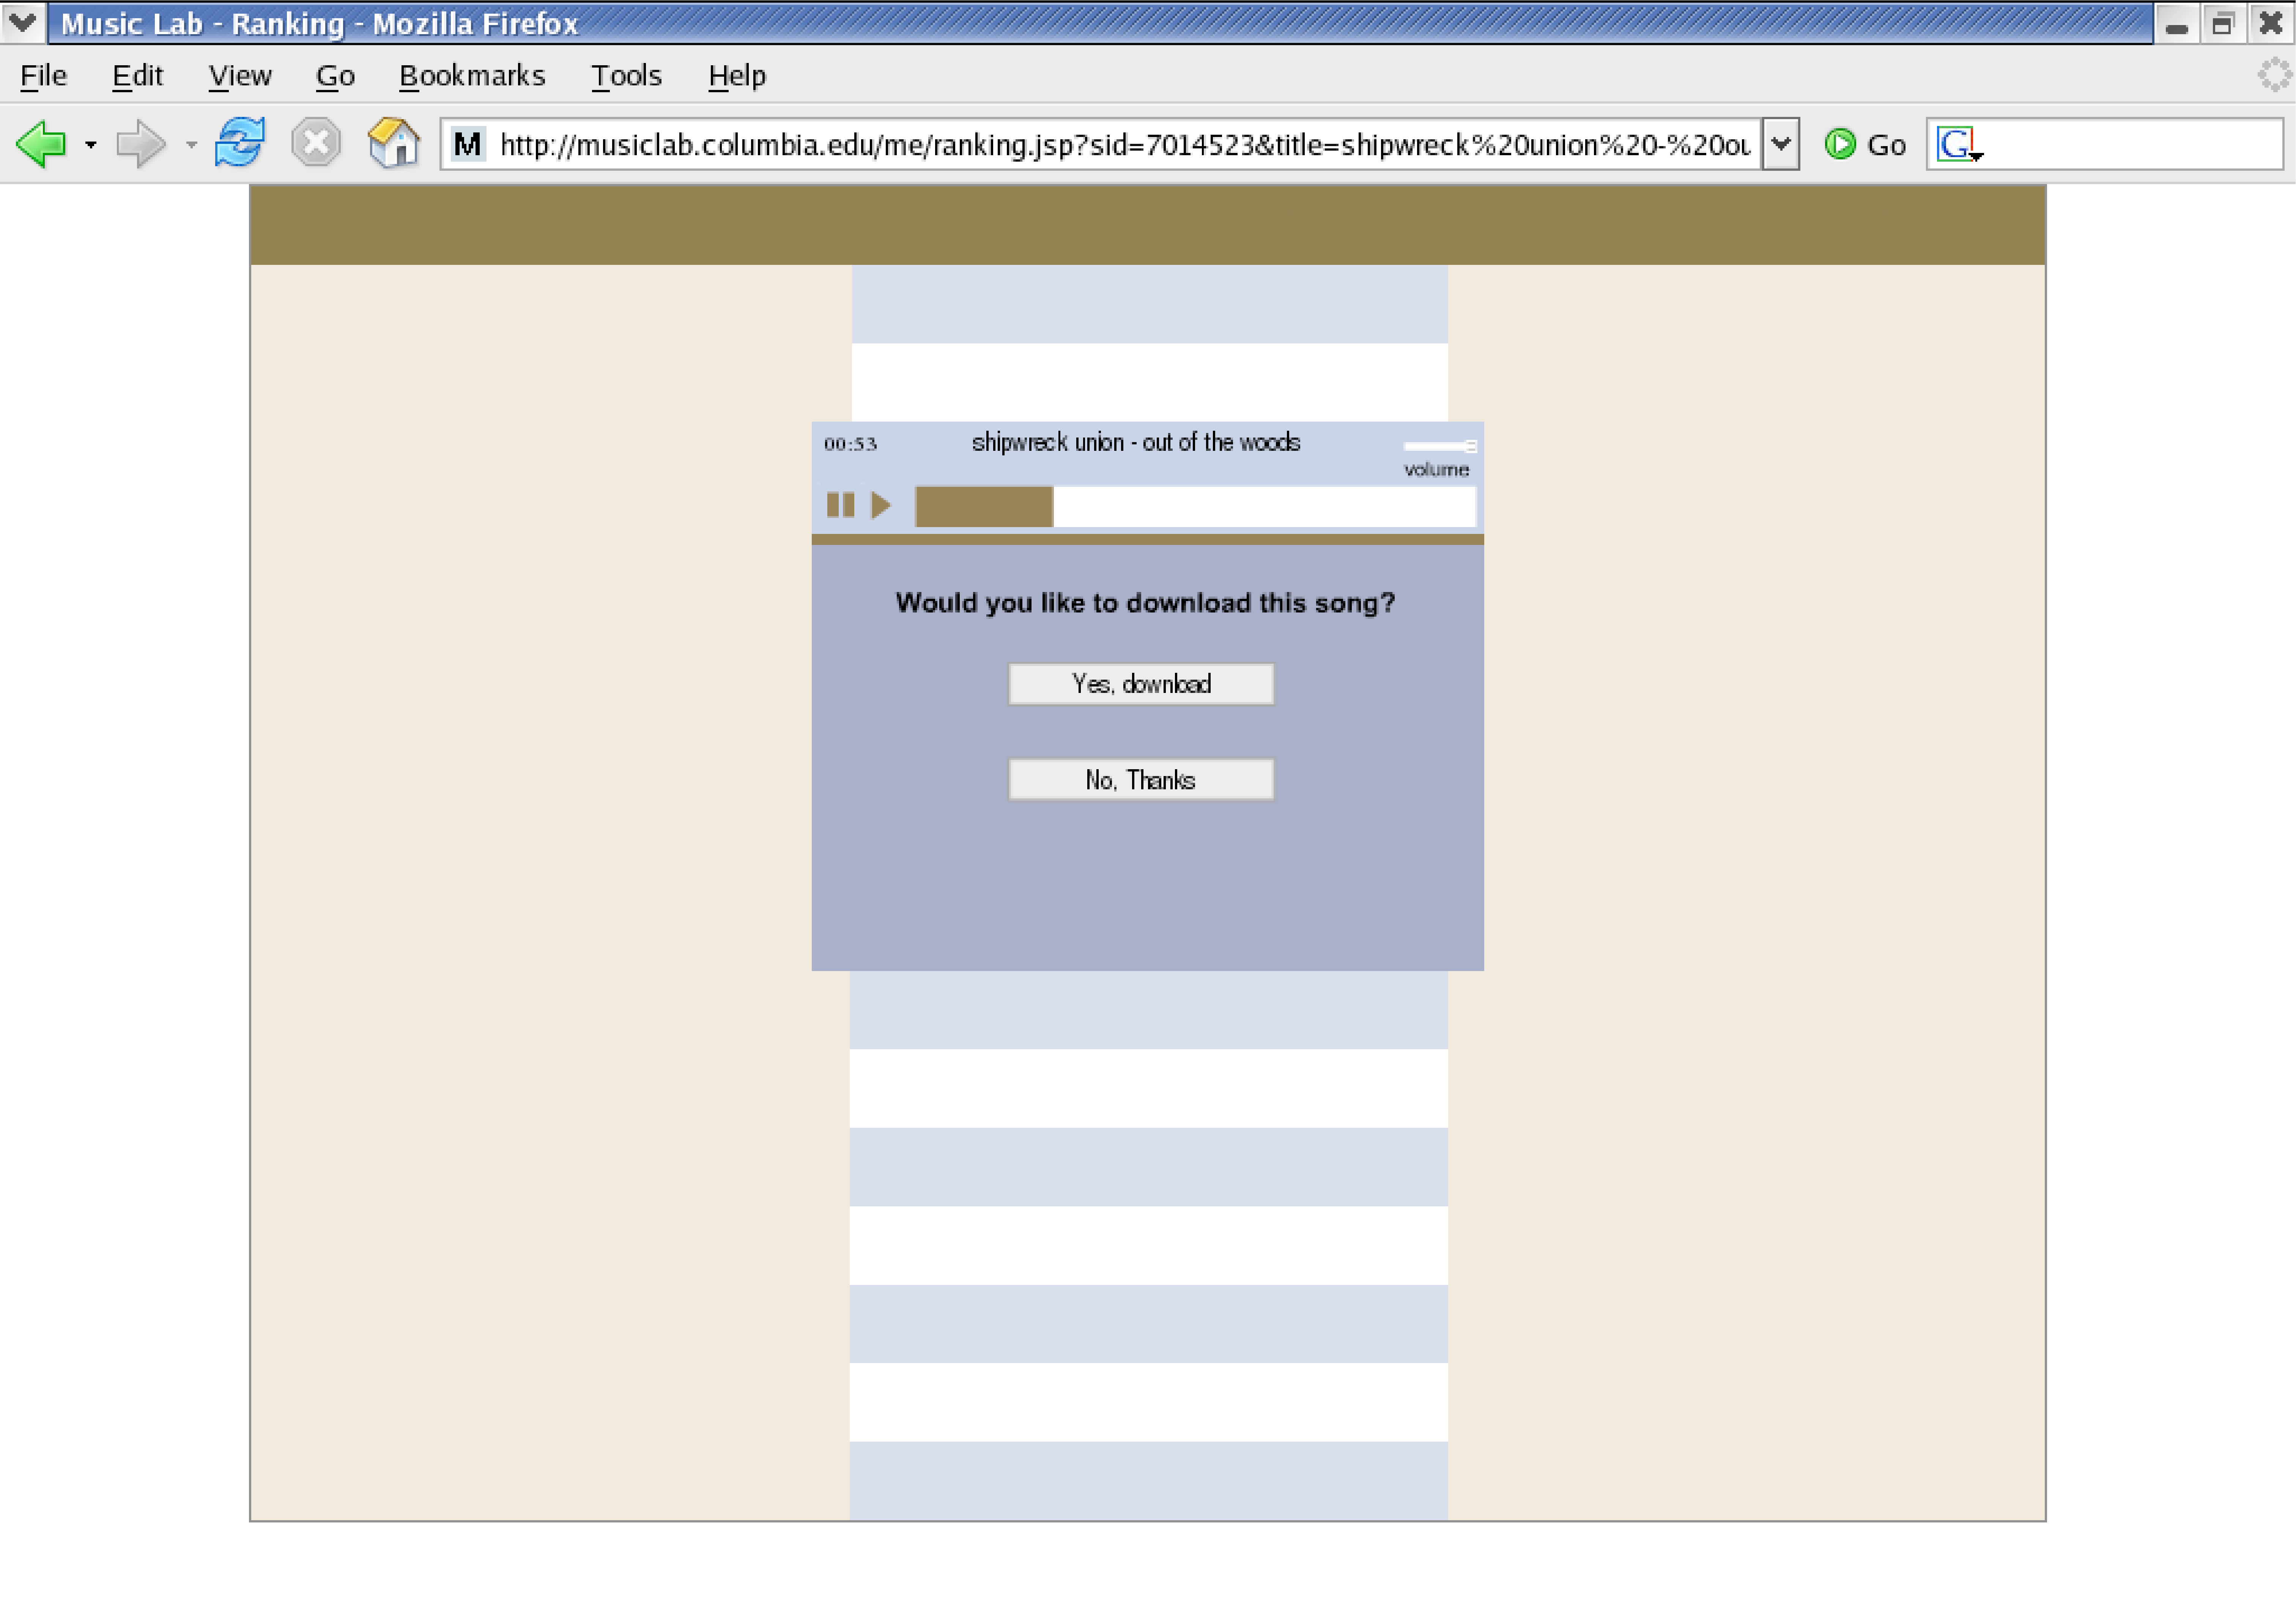
\includegraphics[width = 0.9\textwidth]{figures/downloadscreen}
\end{figure}

\end{frame}
%%%%%%%%%%%%%%%%%%%%%%%%%%%%%%%%%%
\begin{frame}

\begin{figure}
  \centering
  \includegraphics[width = 0.9\textwidth]{figures/info-v1-cut}
\end{figure}

\end{frame}
%%%%%%%%%%%%%%%%%%%%%%%%%%%%%%%%%
\begin{frame}

\begin{itemize}
\item \url{https://www.dropbox.com/s/k02iy1hcw0g3xir/165444-hi.mp3?dl=0}
\item \url{https://www.dropbox.com/s/j0wpjg379xuhe7n/331122-hi.mp3?dl=0}
\item \url{https://www.dropbox.com/s/tobqqk4ar9qzc01/846626-hi.mp3?dl=0}
\end{itemize}

\note{
If time, talk about how to select the sample of songs
}

\end{frame}
%%%%%%%%%%%%%%%%%%%%%%%%%%%%%%%%%
\begin{frame}

\begin{figure}
  \centering
  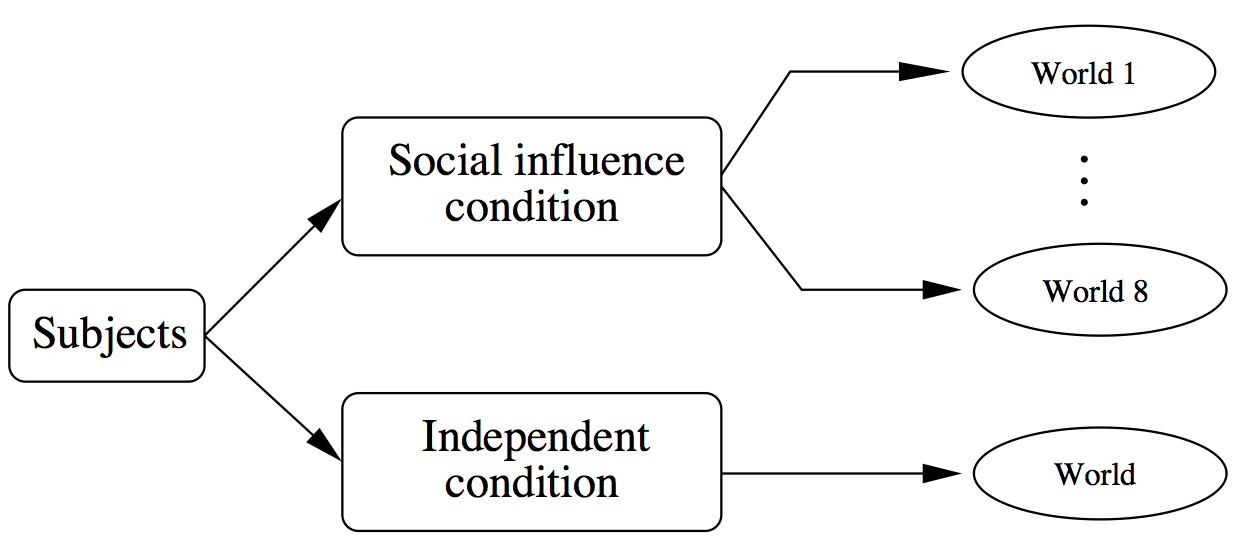
\includegraphics[width=0.9\textwidth]{figures/musiclab_exp_design}
\end{figure}

\end{frame}
%%%%%%%%%%%%%%%%%%%%%%%%%%%%%%%%%
%
%\begin{frame}
%\frametitle{Experiment 1: Screenshots}
%
%\setcounter{subfigure}{0}
%\begin{figure}
%  \centering
%     \subfigure[Social influence condition]{
%     \includegraphics[width=0.45\textwidth]{/Users/matt/projects/musiclab/screenshots/info-v1-cut.eps}}
%  \hspace{0in}
%    \subfigure[Independent condition]{
%     \includegraphics[width=0.45\textwidth]{/Users/matt/projects/musiclab/screenshots/noinfo-v1-cut.eps}}
%\end{figure}
%
%\end{frame}
%%%%%%%%%%%%%%%%%%%%%%%%%%%%%%%%%%
\begin{frame}

\setcounter{subfigure}{0}
\begin{figure}
  \centering
     \subfigure[Experiment 1, Weaker signal]{
     \includegraphics[width=0.45\textwidth]{figures/info-v1-cut}}
  \hspace{0in}
     \subfigure[Experiment 2, Stronger signal]{
     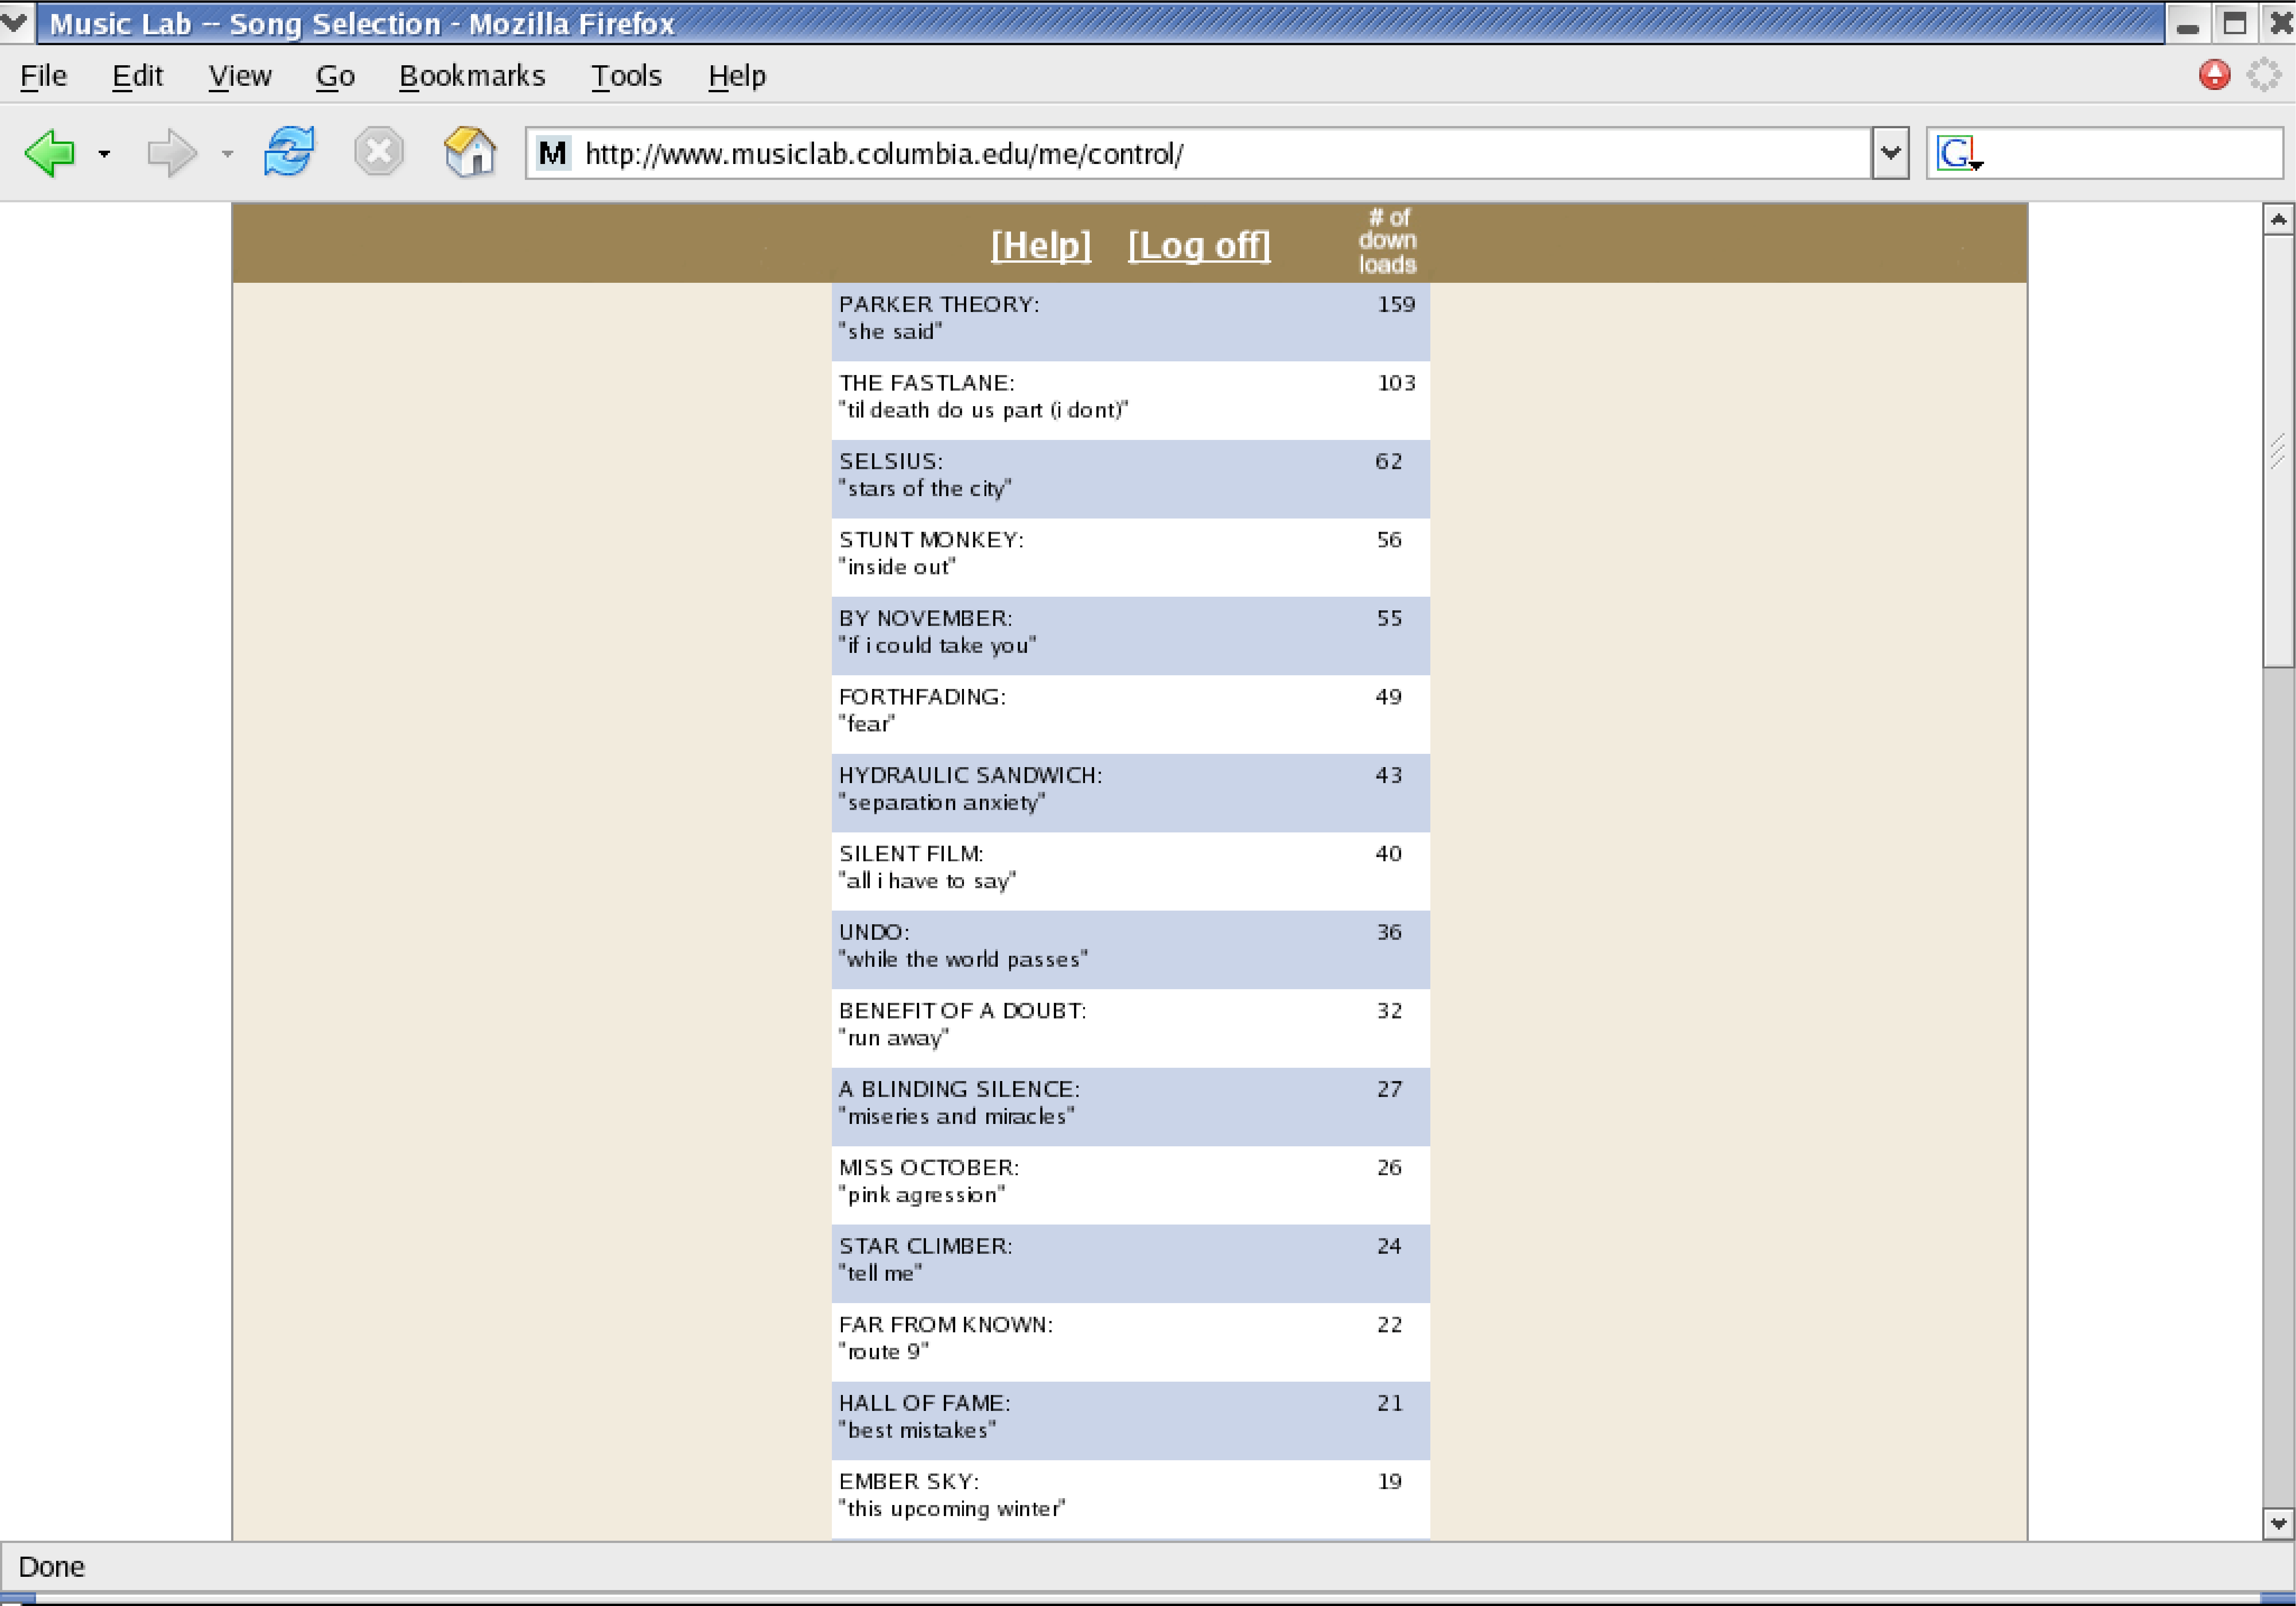
\includegraphics[width=0.45\textwidth]{figures/info-v2}}
\end{figure}

\end{frame}
%%%%%%%%%%%%%%%%%%%%%%%%%%%%%%%%%
%
%\begin{frame}
%\frametitle{Experiment 2: Amplifying the social signal}
%
%December 15, 2004 to March 8, 2005 -- 83 days \\
%Design: 8 social influence worlds, 1 independent world \\
%\vspace{0.4in}
%Summary statistics:
%\begin{itemize}
%  \item 7,192 participants
%  \item 25,860 listens
%  \item 10,298 downloads
%\end{itemize}
%Participants drawn mostly from~\url{http://www.bolt.com}
%\end{frame}
%
%%%%%%%%%%%%%%%%%%%%%%%%%%%%%%%%%
\begin{frame}

\begin{figure}
  \centering
  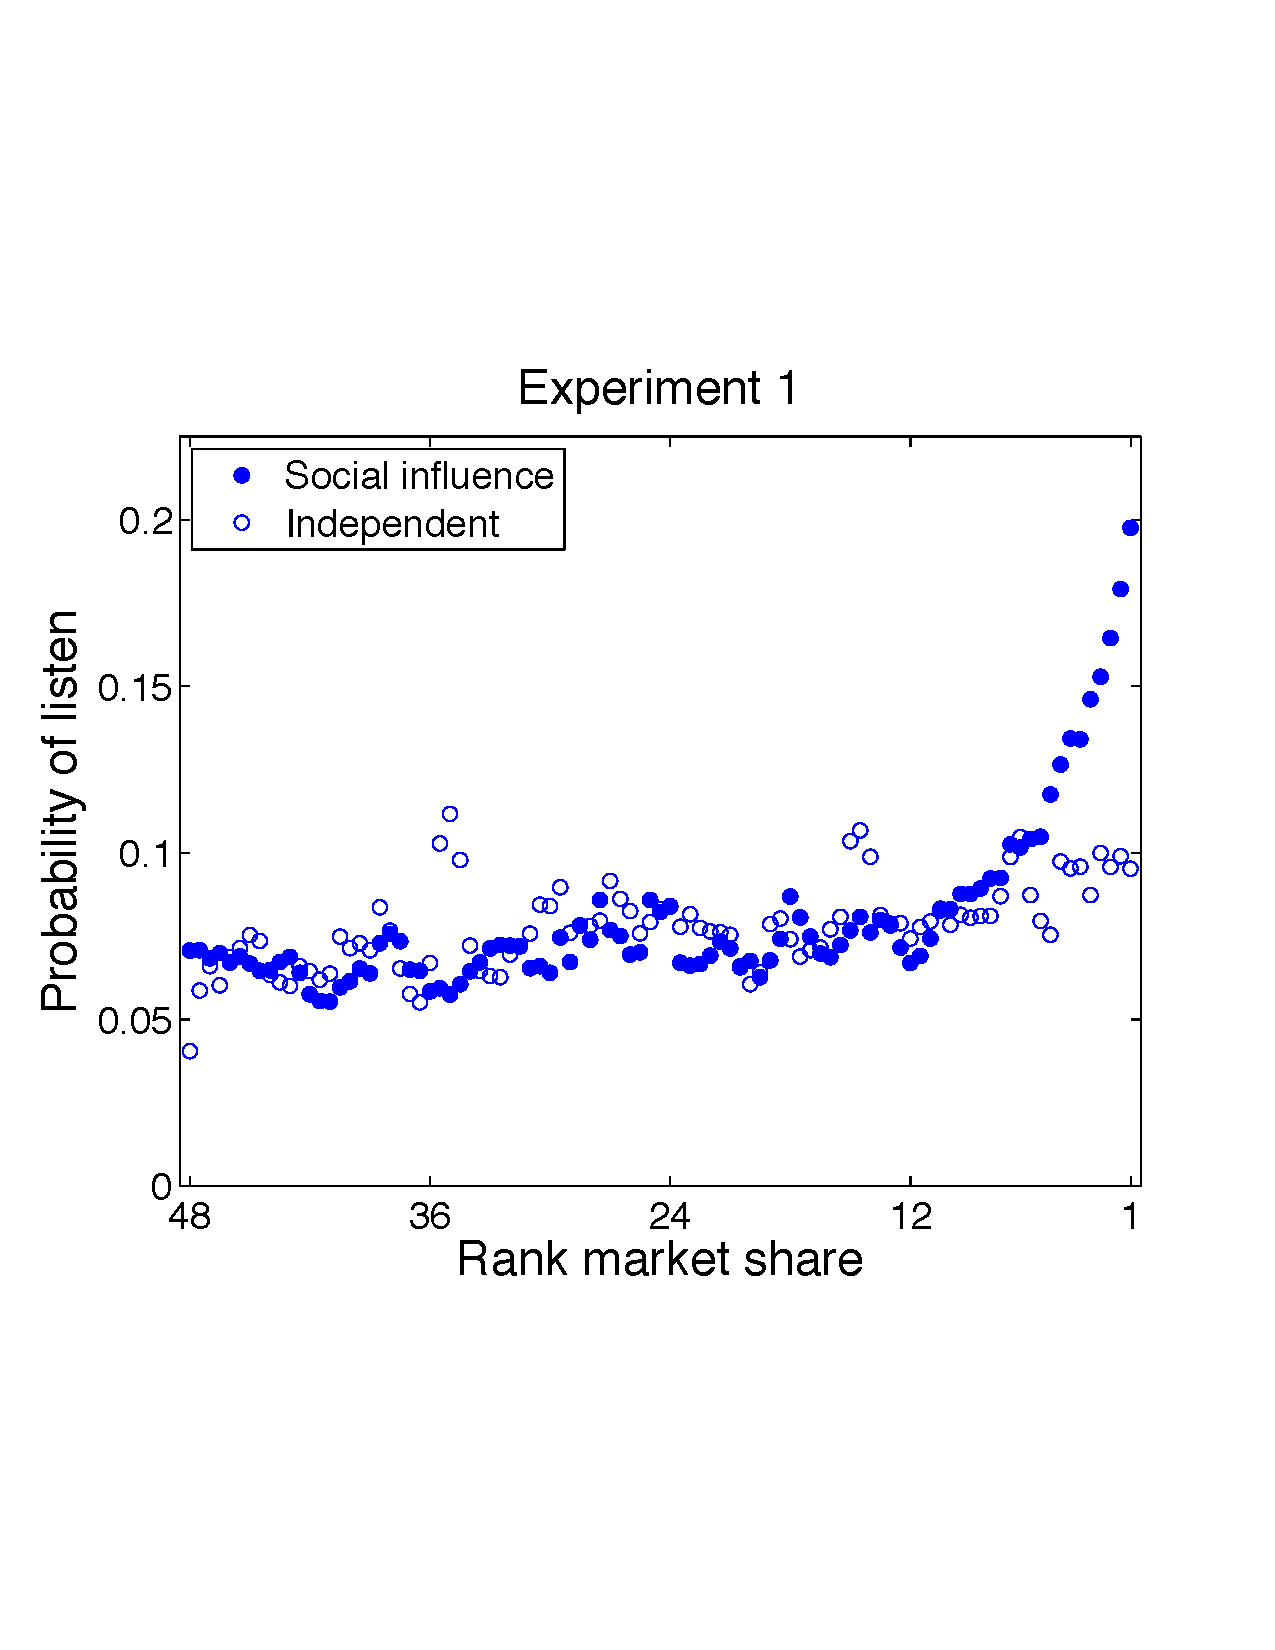
\includegraphics[width= 0.6\textwidth]{figures/listenchoice_v1_smoothed_1}
\end{figure}

\end{frame}
%%%%%%%%%%%%%%%%%%%%%%%%%%%%%%%%%%%%%%%%%%%
\begin{frame}

\setcounter{subfigure}{0}
\begin{figure}
  \centering
     \subfigure[Experiment 1, weaker signal]{
     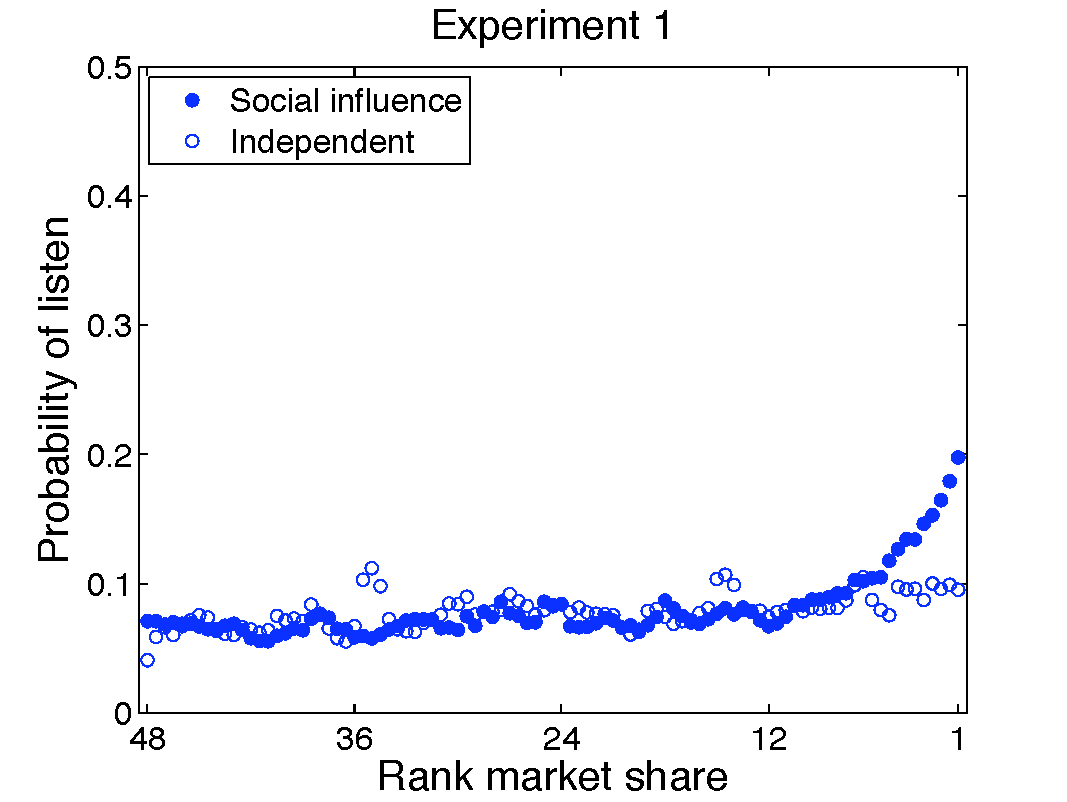
\includegraphics[width=0.45\textwidth]{figures/listenchoice_v1_v2scale_smoothed_1}}
  \hspace{0in}
    \subfigure[Experiment 2, stronger signal]{
     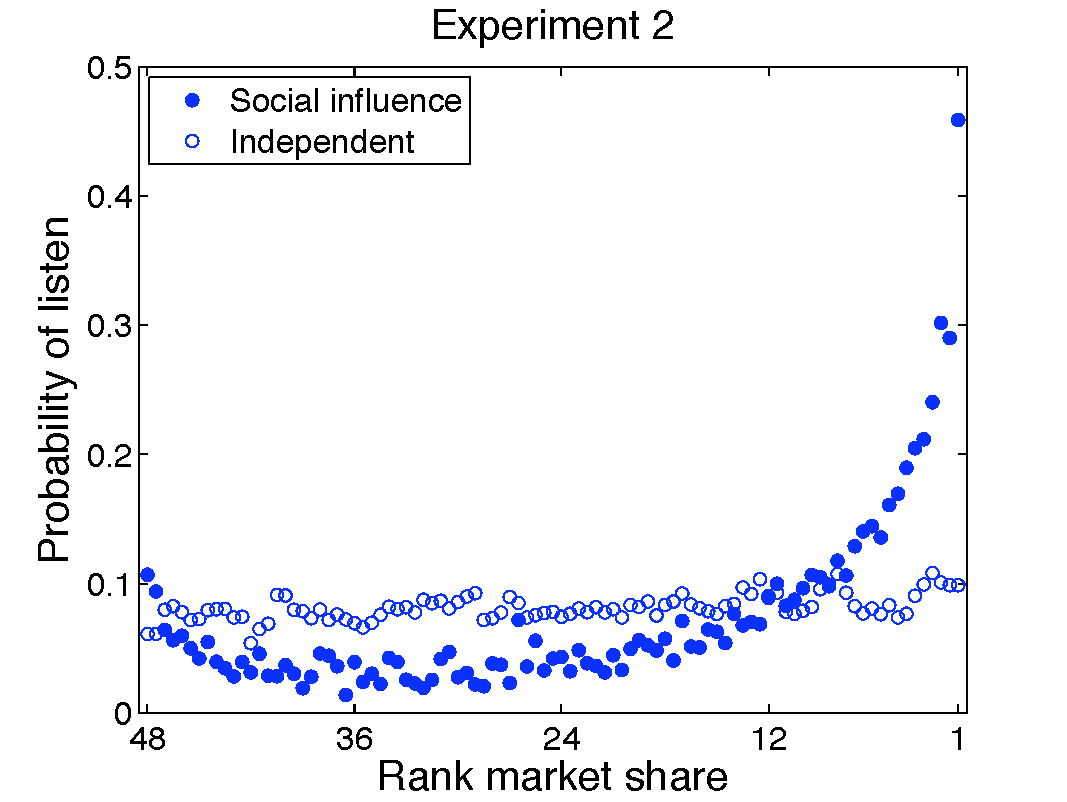
\includegraphics[width=0.45\textwidth]{figures/listenchoice_v2_smoothed}}
\end{figure}

\end{frame}

%%%%%%%%%%%%%%%%%%%%%%%%%%%%%%%%%%
\begin{frame}

\begin{figure}
  \centering
  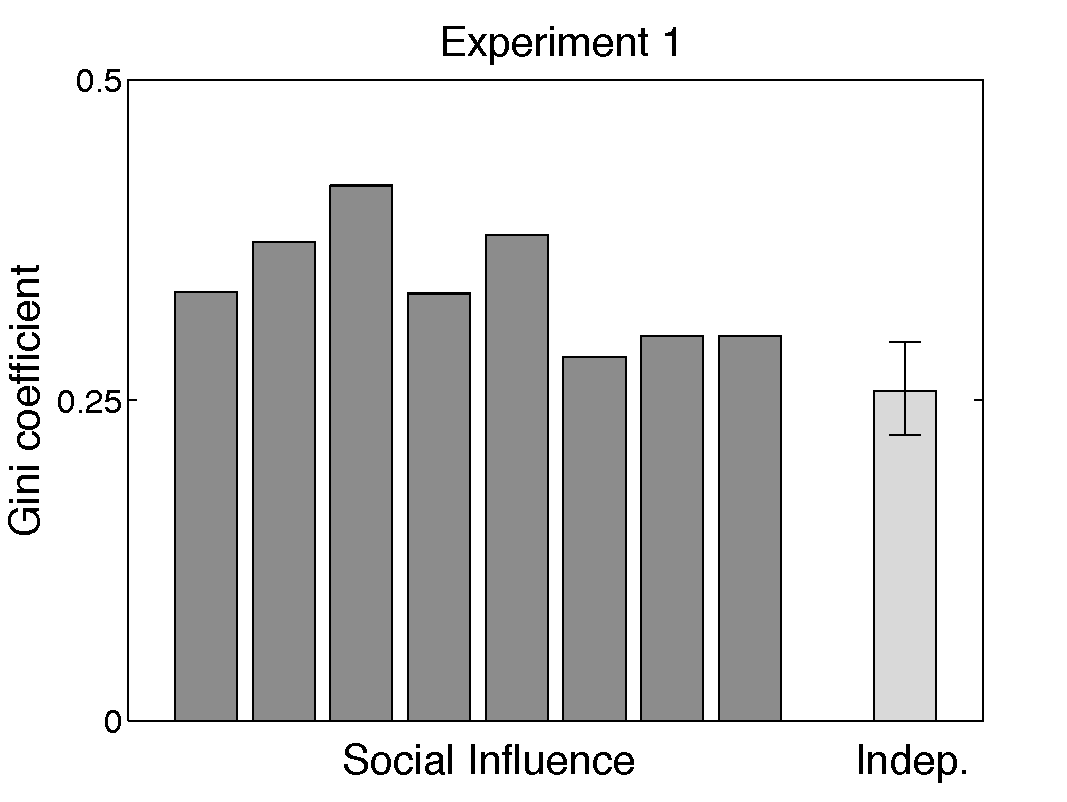
\includegraphics[width=0.7\textwidth]{figures/gini_v1_unordered_ci}
\end{figure}

\end{frame}
%%%%%%%%%%%%%%%%%%%%%%%%%%%%%%%%%%%%%%%%%%%%
\begin{frame}

\begin{figure}
  \centering
  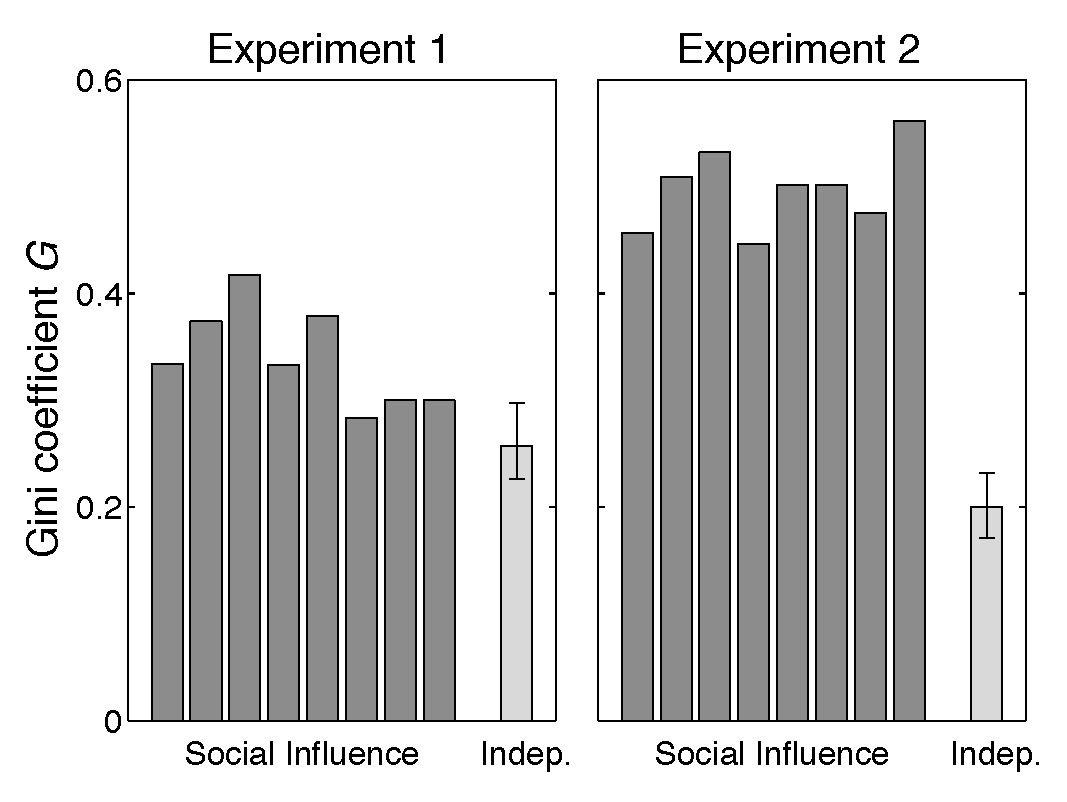
\includegraphics[width=3in]{figures/compare_gini_v1v2_unordered_ci}
\end{figure}

Median Gini coefficient increases from $0.34$ (France) to $0.50$ (Nigeria)
\end{frame}

%%%%%%%%%%%%%%%%%%%%%%%%%%%%%%%%%
\begin{frame}

$U$ = mean difference in market share across all pairs of realizations\\
\begin{figure}
  \centering
  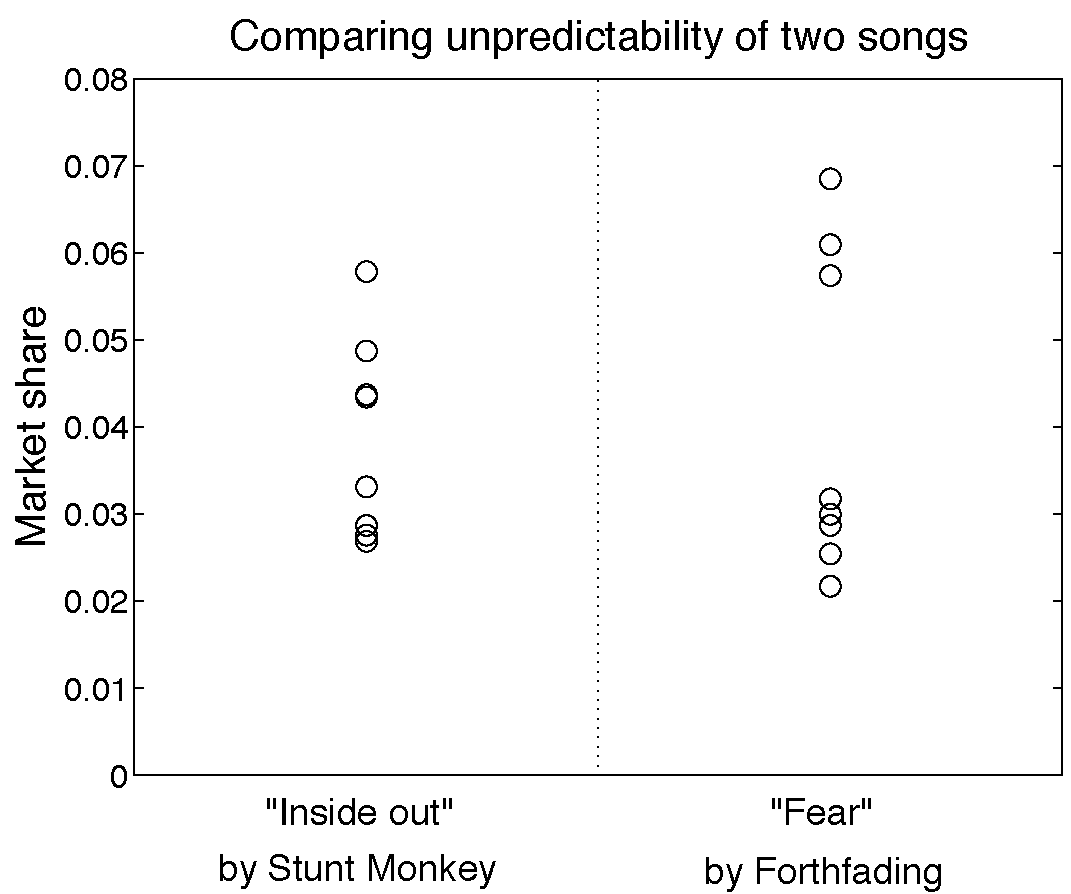
\includegraphics[width = 3in]{figures/arbitrary_example}
\end{figure}

\end{frame}

%%%%%%%%%%%%%%%%%%%%%%%%%%
\begin{frame}

\begin{figure}
  \centering
  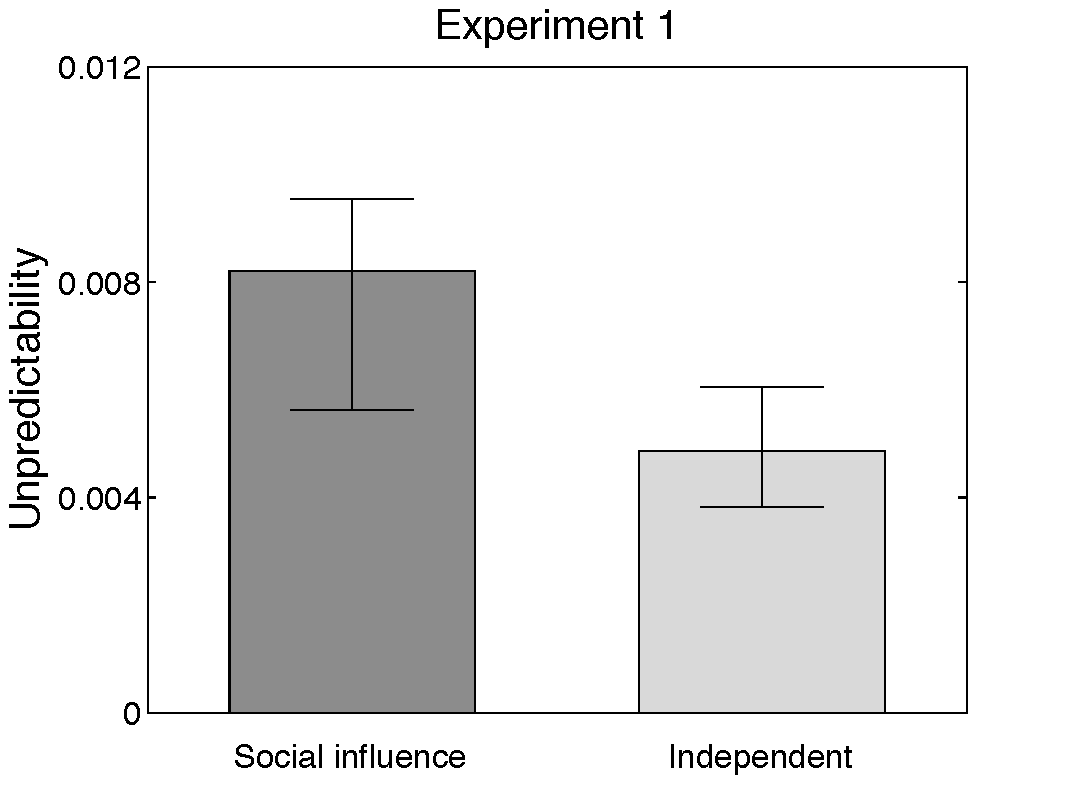
\includegraphics[width = 3.5in]{figures/unpredictability_v1}
\end{figure}

\end{frame}
%%%%%%%%%%%%%%%%%%%%%%%%%%%%
\begin{frame}

\begin{figure}
  \centering
  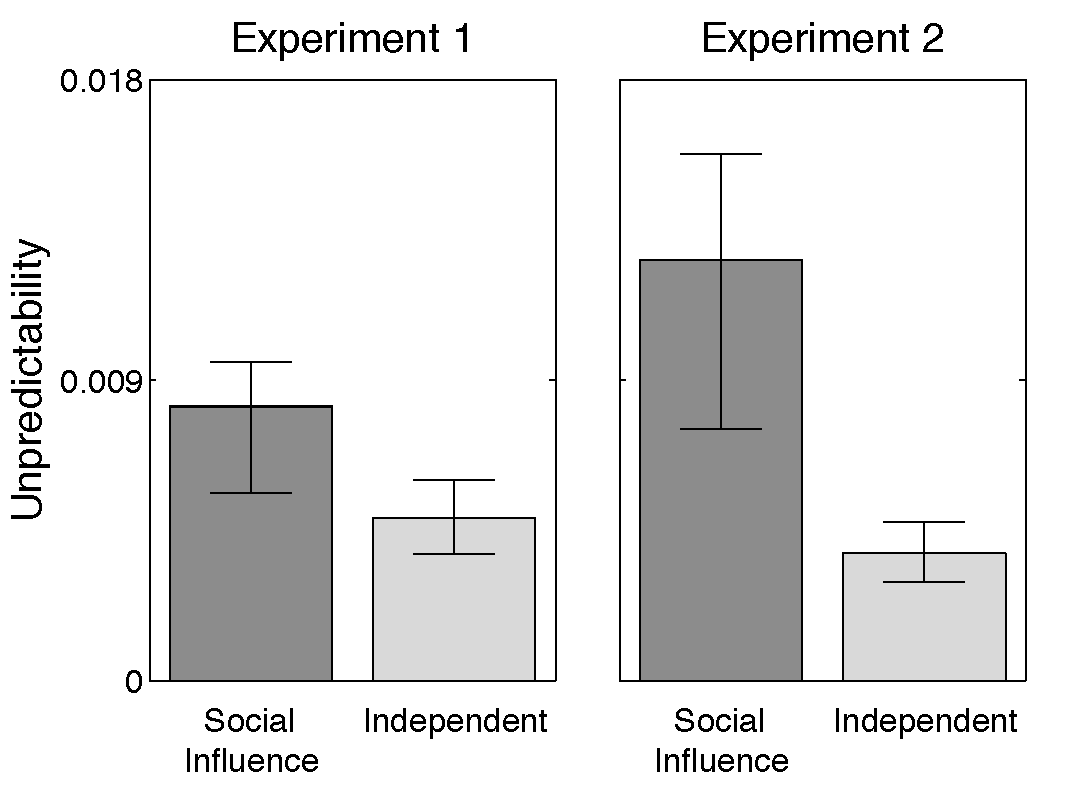
\includegraphics[width=3in]{figures/compare_unpred_v1v2}
\end{figure}

Unpredictability increases by about 50\%
\end{frame}
%%%%%%%%%%%%%%%%%%%%%%%%%%%%%%%%%
\begin{frame}

Experiments 1 and 2 show a dose-response relationship.  Increasing the strength of social influence leads to

\begin{itemize}
  \item increased inequality of success
  \item increased unpredictability of success
\end{itemize}

\vspace{0.4in}
%Increasing the strength of the signal increases the \emph{appearance}
%of predictability while decreasing the \emph{actual} predictability

\end{frame}

%%%%%%%%%%%%%%%%%%%%%%%%%%%%%%%%%
\begin{frame}

What is the relationship between ``quality'' and success?

\end{frame}
%%%%%%%%%%%%%%%%%%%%%%%%%%%%%%%%%%
\begin{frame}

\vspace{0.0in}
\setcounter{subfigure}{0}
\begin{figure}
  \centering
     \subfigure{
     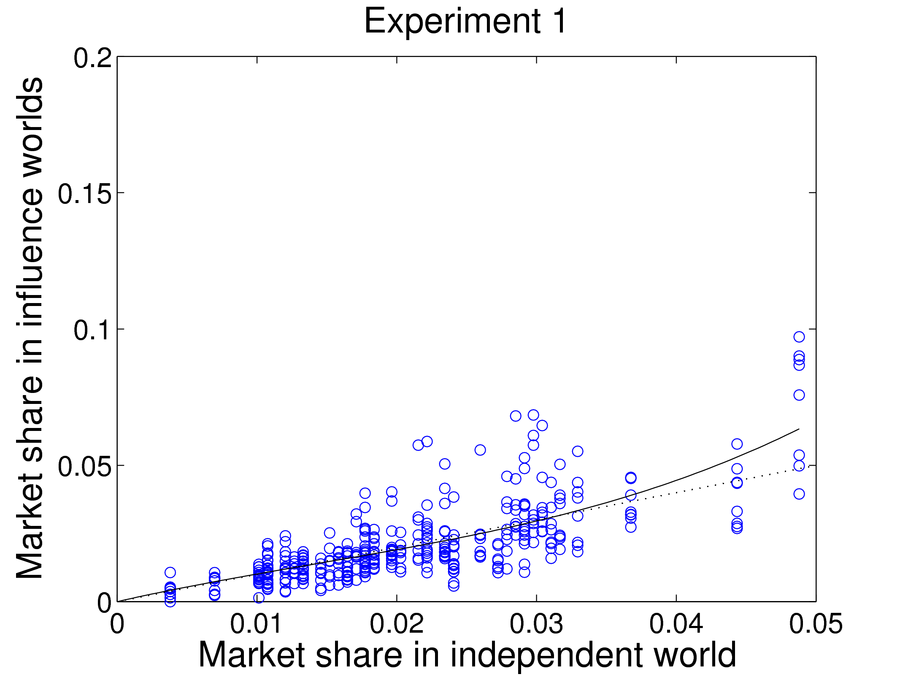
\includegraphics[width=0.45\textwidth]{figures/ms_noinfo_info_v1}}
  \hspace{0in}
     \subfigure{
     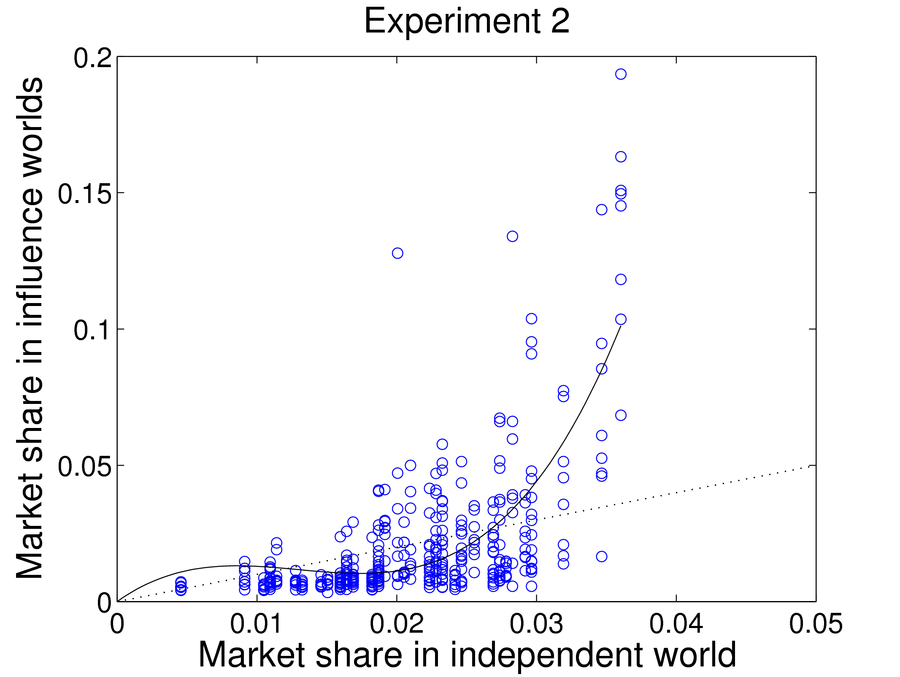
\includegraphics[width=0.45\textwidth]{figures/ms_noinfo_info_v2}}
\end{figure}
 
\end{frame}
%%%%%%%%%%%%%%%%%%%%%%%%%%%%%%%%%%
%
%\begin{frame}
%\frametitle{Relationship between ``quality'' and success: ranks}
%
%\vspace{0.0in}
%\setcounter{subfigure}{0}
%\begin{figure}
% \centering
%     \subfigure{
%     \includegraphics[width=0.45\textwidth]{/Users/matt/projects/musiclab/figures/ms_noinfo_info_v1_rank.eps}}
%  \hspace{0in}
%     \subfigure{
%     \includegraphics[width=0.45\textwidth]{/Users/matt/projects/musiclab/figures/ms_noinfo_info_v2_rank.eps}}
%\end{figure}
% 
%Highest ``quality'' songs never do terrible, lowest ``quality'' never do great, any other result possible\\
%
%\end{frame}
%
%%%%%%%%%%%%%%%%%%%%%%%%%%%%%%%%%%%%
\begin{frame}

If real success can lead to more success, can fake success lead to real success?


\end{frame}
%%%%%%%%%%%%%%%%%%%%%%%%%%%%%%%%%%

\end{document}
